\documentclass[a4paper,12pt,hidelinks]{book} 

\usepackage[hmargin=1in, vmargin=1in]{geometry}

\usepackage[hidelinks]{hyperref}

\usepackage{amsthm, amssymb}

\usepackage[fleqn]{amsmath}
\setlength{\mathindent}{1cm}

\usepackage{algorithm}
\usepackage{algpseudocode}
\newcommand{\BlockComment}[1]{\vspace{1em}\Statex \textbf{#1}}

\usepackage{graphicx}
\usepackage{array}
\usepackage[export]{adjustbox}
\usepackage{caption}
\usepackage{parskip}

\usepackage{tikz}
\usetikzlibrary{positioning}
\usetikzlibrary{arrows.meta}

\usepackage{pgfplots}
\pgfplotsset{compat=newest}

%\includeonly{2_Improving_deep_neural_networks_3.tex}

\setcounter{tocdepth}{1}

\begin{document}

\tableofcontents

\part{Neural Networks and Deep Learning}
\include{1_Neural_networks_and_deep_learning.tex}

\part{Improving Deep Neural Networks}
% -----------------------------------------------------
% CHAPTER 1
% -----------------------------------------------------

\chapter{Week 1 \\ Practical Aspects of Deep Learning}







% - Setting up your Machine Learning Application --------------------------------

\section{Setting up your Machine Learning Application}

\subsection*{Train/Dev/Test Sets}

\begin{itemize}
    \item \textbf{Training set}: used to train the model
    \item \textbf{Dev/cross validation set}: used to evaluate the model and tune hyperparameters
    \item \textbf{Test set}: used to evaluate the model
\end{itemize}

\subsection*{Set Sizes}

How a data set is split into train/dev/test depends on the size of the data set. Here are some examples: 

\begin{tabular}[t]{|l|r|r|r|}
    \hline
    m & train & dev & test \\
    \hline
    $<10,000$ & $70$ & $30$ & \\
    \hline
    $<10,000$ & $60$ & $20$ & $20$\\
    \hline 
    $>1,000,000$ & $98$ & $1$ & $1$\\
    \hline
\end{tabular}

\subsection*{Mismatching train/test sets}

\begin{itemize}
	\item Do the training on one distribution of data that might be easier to gather, or consists of synthetic data, augmented data etc., then do testing on a different distribution.
	\item Test and dev should be from the same distribution.
    \item It may be OK to not use a test set, but just work with train \& dev cross validation.
\end{itemize}






% - Bias/Variance ---------------------------------------------------------------

\section{Bias \& Variance}

\begin{figure}[htbp] % 'htbp' is a placement specifier; it means "here, top, bottom, page"
    %\centering
    
    \begin{minipage}[t]{0.3\textwidth}
        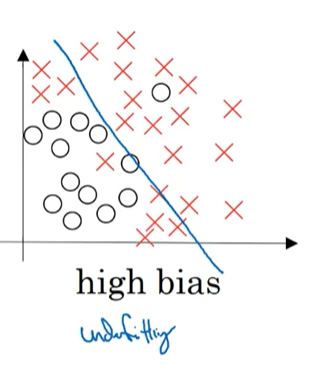
\includegraphics[width=\linewidth, valign=t]{images/high_bias.png}
    \end{minipage}
    \hfill % This will create horizontal space between the images
    \begin{minipage}[t]{0.3\textwidth}
        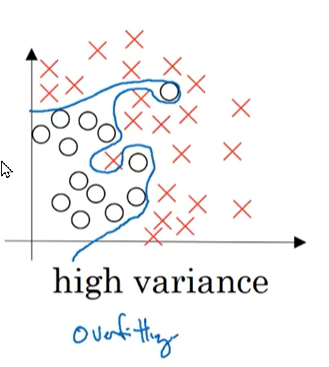
\includegraphics[width=\linewidth, valign=t]{images/high_variance.png}
    \end{minipage}
    \hfill
    \begin{minipage}[t]{0.3\textwidth}
        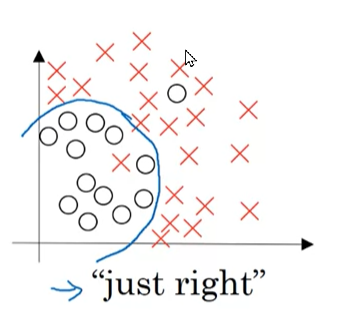
\includegraphics[width=\linewidth, valign=t]{images/low_b_v.png}
    \end{minipage}
    
\end{figure}


Given an optimal error of $0\%$

\begin{tabular}[t]{|l|l|l|l|l|}
    \hline
    Train Error & $1\%$ & $15\%$ & $15\%$ & $0.5\%$ \\
    \hline
    Dev Error & $11\%$ & $16\%$ & $30\%$ & $1\%$ \\
    \hline
    & 
    \begin{tabular}{l}
        High variance \\
        Overfitting
    \end{tabular}
    &
    \begin{tabular}{l}
        High bias\\
        Underfitting
    \end{tabular}
    &
    \begin{tabular}{l}
        High bias,\\ 
        variance
    \end{tabular}
    &
    \begin{tabular}{l}
        Low bias,\\ 
        variance
    \end{tabular}
    \\
    \hline
\end{tabular}

\begin{figure}[htbp] % 'htbp' is a placement specifier; it means "here, top, bottom, page"
    \begin{minipage}[t]{0.3\textwidth}
        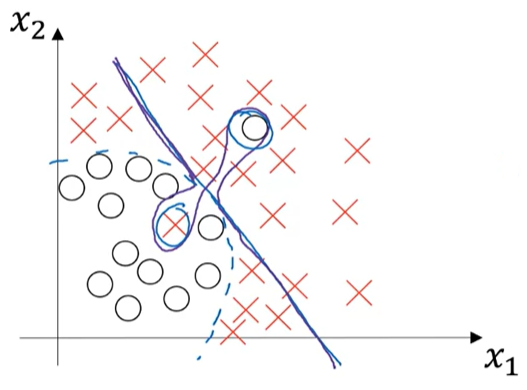
\includegraphics[width=\linewidth, valign=t]{images/high_b_v.png}
        \caption*{High bias, high variance}
        \label{fig:high_b_v}
    \end{minipage}
\end{figure}

This seems like a contrived example in two dimensions, but in higher dimensions its more plausible.

\subsection*{Basic Recipe for Machine Learning}

If high bias (underfitting):
\begin{itemize}
    \item bigger network
    \item train longer
    \item different NN architecture
\end{itemize}

If high variance (overfitting):
\begin{itemize}
    \item more data
    \item regularization
    \item different NN architecture 
\end{itemize}
    
Rinse and repeat until low bias \& variance.There's not much trade off between bias and variance in deep learning

\newpage





% -- Regularizing your Neural Network ------------------------------------------

\section{Regularizing your Neural Network}

\subsection*{Adding a Regularization Term}

\subsubsection*{Logistic regression}

\[ \underset{(w, b)}{min} \in J(w, b) \]
\[ w\in\mathbb{R}^{n_x}$, $b\in\mathbb{R} \]
\[ J(w,b)=\frac{1}{m} \sum_{i=1}^{m}\mathcal{L}(\hat{y}^{(i)}, y^{(i)}) \]

Add regularization (L2-regularization)
\[ \mathcal{J}(w,b)=\frac{1}{m} \sum_{i=1}^{m}\mathcal{L}(\hat{y}^{(i)}, y^{(i)})+ \frac{\lambda}{2m} \|w\|_2^2 \]

where
\[ \|w\|_2^2=\sum_{j=1}^{n_x}w_j^2=w^Tw \]


Add regularization (L1-regularization)

\[ \mathcal{J}(w,b)=\frac{1}{m} \sum_{i=1}^{m}\mathcal{L}(\hat{y}^{(i)}, y^{(i)})+ \frac{\lambda}{2m} \|w\|_1 \]

where
\[ \|w\|_1 = \sum_{j=1}^{n_x}|w_j| \]

L1-regularization can lead to w becoming sparse

$\lambda$ is called the regularization parameter

We could add a regularization term on b as well, but has little effect compared to the w-based term.

\subsubsection*{Neural Network}

Add regularization term over all layers' parameters:
\[ 
    \mathcal{J}(w^{[1]}, b^{[1]}, \ldots, w^{[L]} , b^{[L]} )=\frac{1}{m} \sum_{i=1}^{m}\mathcal{L}(\hat{y}^{(i)}, y^{(i)})+ 
    \frac{\lambda}{2m}\sum_{l=1}^L\|w^{[l]}\|_F^2 
\]

$w$ is a $(n^{[l]} , n^{[l-1]})$ matrix, and the "L2-norm" of a matrix is called the Frobenius norm. 
For a layer $l$ the norm is:
\[ \|w^{[l]}\|_F^2= \sum_{i=1}^{n^{[l-1]}} \sum_{j=1}^{n^{[l]}}({w_{ij}}^{[l]})^2 \]

\subsubsection*{Gradient descent with regularization}

\begin{align}
    dw^{[l]}= & (\text{from backprop})+ \frac{\lambda}{m} w^{[l]} \\
    w^{[l]} = & w^{[l]} - \alpha dw^{[l]} \\
            = & w^{[l]} - \alpha( (\text{from backprop}) + \frac{\lambda}{m}w^{[l]} ) \\
            = & w^{[l]} - \alpha \frac{\lambda}{m} w^{[l]} - \alpha(\text{from backprop})
\end{align}


The second term has the effect of reducing the size of $w$ slightly, 
which is why this regularization is also called "weight decay."

\subsubsection*{How does regularization prevent overfitting?}

Intuition: With a large value for $\lambda$, the $w^{[i]}$  will be brought to $\approx${0}, 
in effect zeroing out the effect of some nodes in the network, bringing the variance down. 
In practice, the weights won't be 0, but the values will be smaller.
\[ \lambda \uparrow \implies w^{[l]} \downarrow\]

so then
\[ z^{[l]} = w^{[l]}  a^{[l-1]} + b \]

will be small, and so the activation function
\[ g(z)=tanh(z) \]

will be close to linear for those values of $z$, and the network will behave more like a linear network: 

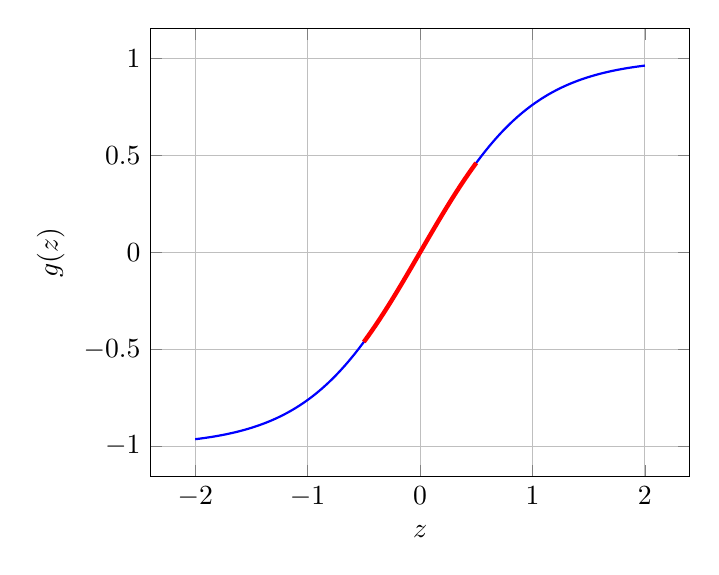
\begin{tikzpicture}
    
    \begin{axis}[
        xlabel={\( z \)},
        ylabel={\( g(z) \)},
        grid=major,
        %title={tanh activation function, \( g(z) = \tanh(z) \)},
        domain=-2:2,
        samples=100,
    ]
    \addplot[blue, thick] {tanh(x)};
    \addplot[red, ultra thick, domain=-0.5:0.5] {tanh(x)};

    %\legend{\( g(z) = \tanh(z) \), almost linear part}
    \end{axis}
\end{tikzpicture}




\newpage

\subsection*{Dropout regularization}

\begin{figure}[htbp]
    \begin{minipage}[t]{\textwidth}
        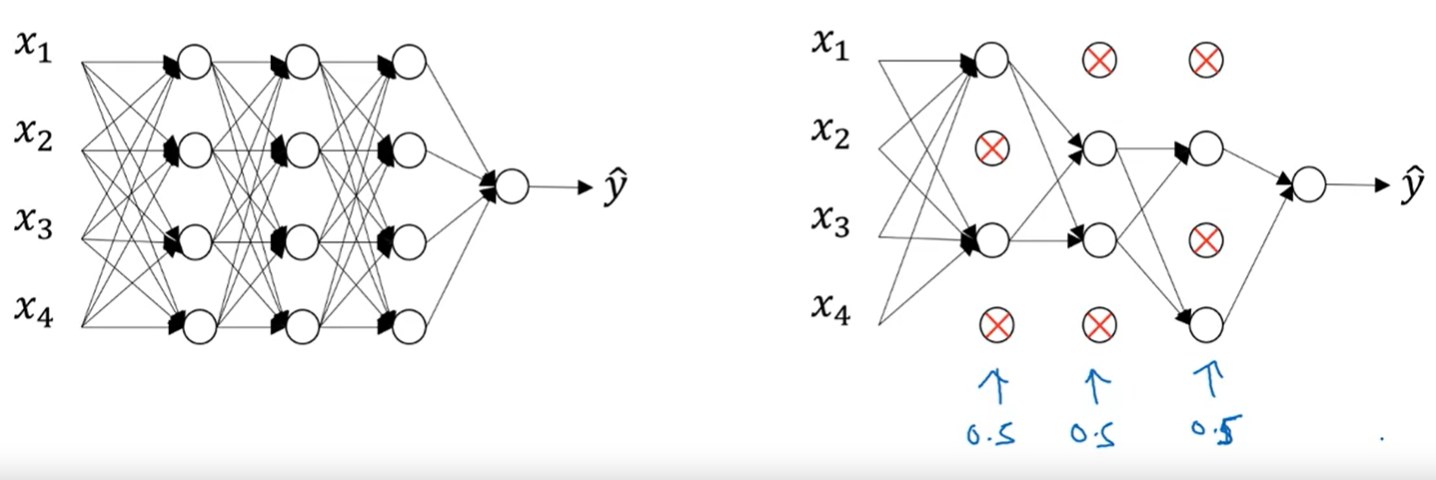
\includegraphics[width=\linewidth, valign=t]{images/dropout.png}
        \caption*{Dropout}
    \end{minipage}
\end{figure}

\subsubsection*{Implementing dropout}

\begin{algorithm}[H]
    \caption*{Inverted dropout}
    \begin{algorithmic}[1]
        \BlockComment{Probability of keeping a node active}
        \State $keep\_prob = \ldots$
        \BlockComment{Vector of bools}
        \State $d^{[l]} = np.random.rand(a^{[l]}.shape[0], a^{[l]}.shape[1]) < keep\_prob$
        \BlockComment{Keep the nodes where d is True only}
        \State $a^{[l]} = np.multiply(a^{[l]}, d^{[l]})$
        \BlockComment{Scale the result}
        \State $a^{[l]} /= keep\_prob$
    \end{algorithmic}
\end{algorithm}

The last line is to scale a3 back to the expected size when used in the activation function, 
and also keeps it in line with the size used in inference, when dropout is not employed.

Intuition: Can't rely on any one feature, so have to spread out the weights $\implies$ smaller weights, 
similar to L2 regularization.

It may be a good idea to have different values for $keep\_prob$ for different layers:
\begin{itemize}
    \item low for the larger ones (many inputs and outputs) where overfitting is more likely a risk, 
    \item higher for others, up to 1.0 (no dropout) for the smallest layers. 
\end{itemize}


\textbf{Downsides}:
\begin{itemize}
    \item increases the number of hyperparameters to find good values for.
    \item the cost function $\mathcal{J}(w, b)$ is no longer well defined. 
        This means the graph of loss x training iteration becomes less meaningful.
\end{itemize}

\newpage

\subsection*{Other regularization methods}

\subsubsection*{Data augmentation}

If you can't collect more data, try augmenting existing data with variations, 
e.g. by flipping or random rotation, distortion and/or cropping of images. 
This will not add as much information as collecting more data,
but will give your algorithm more data and therefore sort of regularize it and reduce over fitting.

\begin{figure}[htbp]
    \begin{minipage}[t]{\textwidth}
        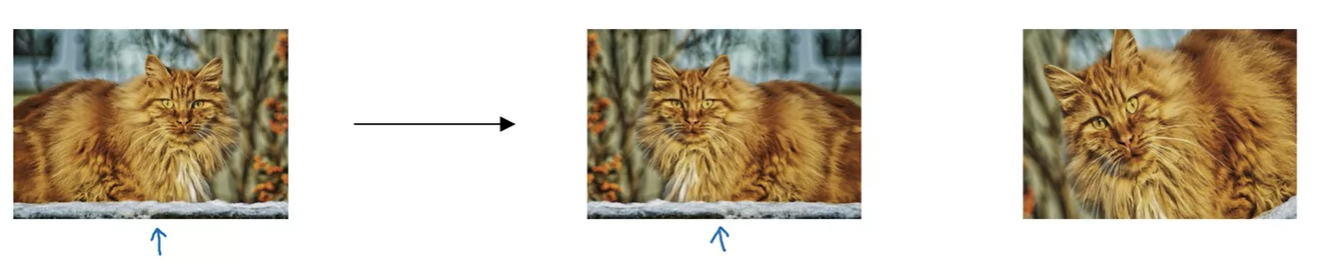
\includegraphics[width=\linewidth]{images/augmented_catpic.png}
    \end{minipage}
\end{figure}

\subsubsection*{Early stopping}

Stopping when dev set error is at a minimum.

\begin{figure}[htbp]
    \begin{minipage}[t]{\textwidth}
        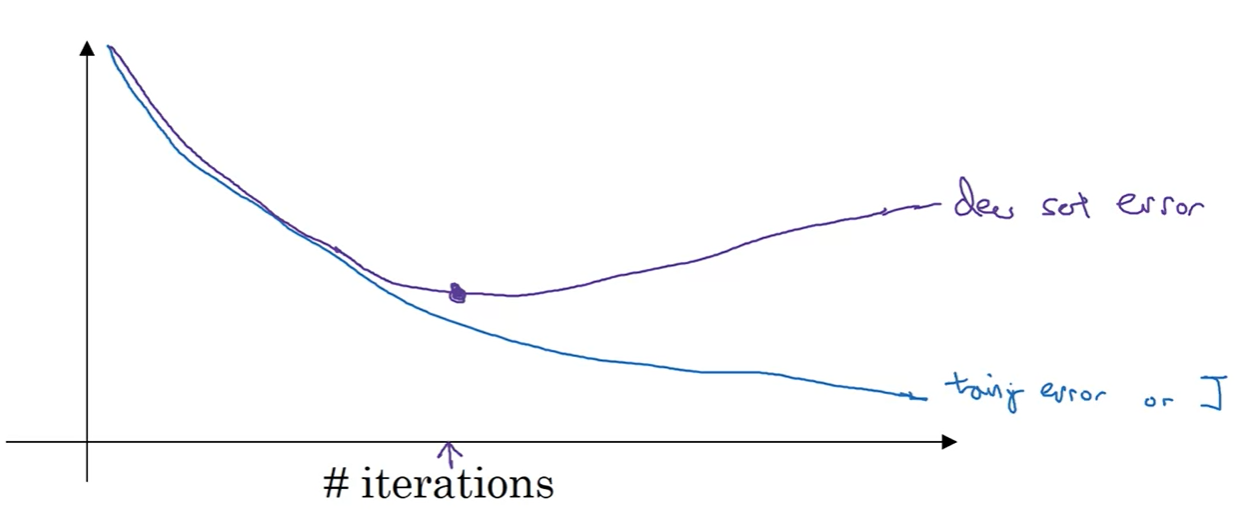
\includegraphics[width=\linewidth]{images/early_stopping.png}
    \end{minipage}
\end{figure}

When you haven't run many iterations, $w\approx0$. During training, the values of w will increase,
so on the right part of the x-axis above, values for w will be large. At the mid point in the graph, 
the value for $\|w\|_F^2$  will be ``mid-sized''. So by picking this version of the network, 
you will get a network with smaller weights, much like one trained with L2-regularization.

\textbf{Downside}: Breaking orthogonality between optimizing $\mathcal{J}(w, b)$ and avoiding overfitting. 
In ML, we can otherwise view these two concepts as orthogonal:

\begin{itemize}
	\item Optimize cost function $\mathcal{J}(w, b)$, using
	\begin{itemize}
		\item Gradient descent
		\item Adam
		\item ...
    \end{itemize}
	\item Avoid overfitting by
    \begin{itemize}
        \item regularization
		\item more data
		\item ...
    \end{itemize}
\end{itemize}

%\newpage





% -- Setting Up your Optimization Problem ---------------------------------------

\section{Setting Up your Optimization Problem}

\subsection*{Normalizing Inputs}

\begin{figure}[htbp]
    \centering
    \begin{minipage}[t]{0.6\textwidth}
        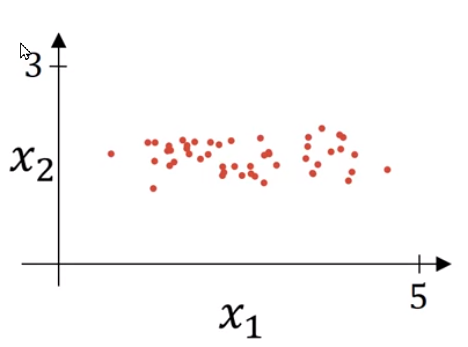
\includegraphics[width=\linewidth]{images/data_not_normalized.png}
    \end{minipage}
\end{figure}


\begin{tabular}{c|c}

    Subtract the mean: &
    Normalize variance: \\

    & \\

    \mbox{$\displaystyle \mu = \frac{1}{m} \sum_{i=1}^m x^{(i)} $} &
    \mbox{$\displaystyle \sigma^2 = \frac{1}{m} \sum_{i=1}^{m} (x^{(i)} - \mu)^2 $} \\

    & \\

    \fbox{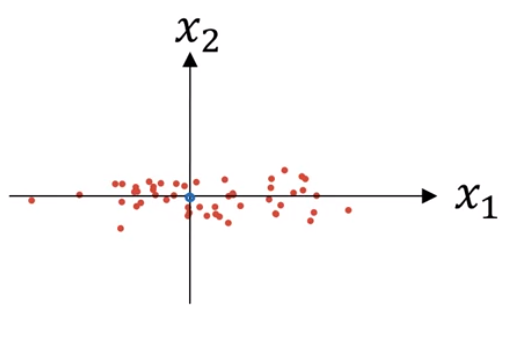
\includegraphics[width=0.4\textwidth]{images/data_mean_subtracted.png}} &
    \fbox{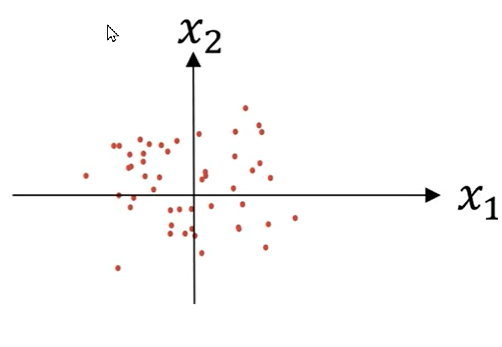
\includegraphics[width=0.4\textwidth]{images/data_normalized.png}} \\

    plot of $x - \mu$ &
    plot of $\frac{x - \mu}{\sigma}$ \\

    & \\

\end{tabular}

Scale the test set in the same way as the training set, with the same values for $\sigma$ and $\mu$.

\newpage

\subsection*{Why Normalize inputs?}

Plotting the cost function 

\[ \mathcal{J}(w, b)= \frac{1}{m} \sum_{i=1}^m \mathcal{L}(\hat{y}^{(i)}, y^{(i)}) \]

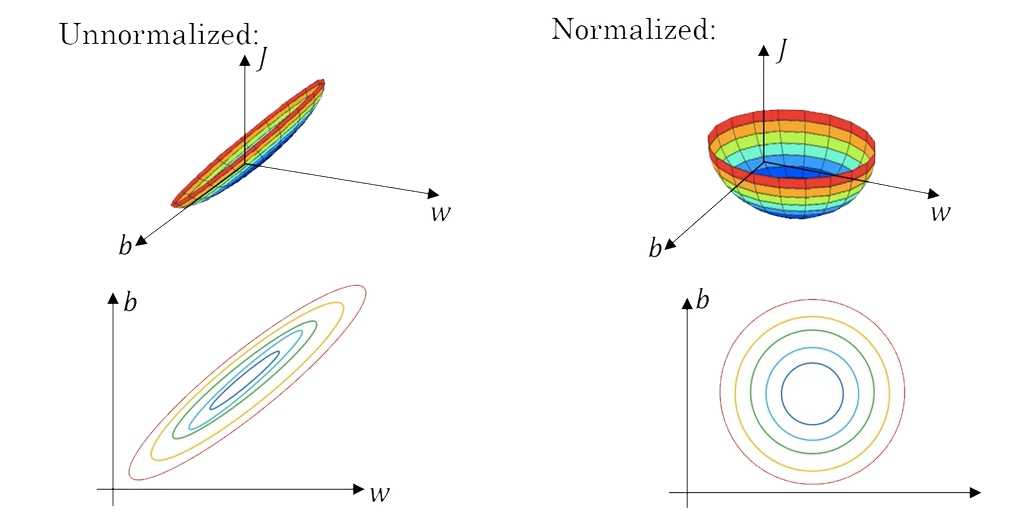
\includegraphics{images/normalized_cost_function.png}

In the non-normalized case, we may need a very small learning rate to avoid gradient descent jumping around all over the place,
whereas in the normalized case we can use a larger learning rate and the network can converge faster without oscillating:

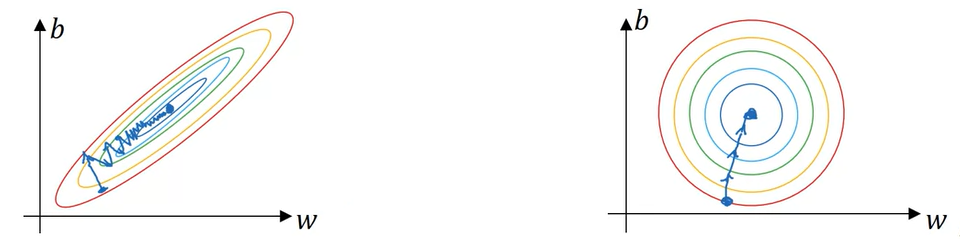
\includegraphics{images/normalized_gd.png}

\subsection*{Vanishing or Exploding Gradients}

During training of a deep network, gradients may grow exponentially large or small, making training difficult.

Example:

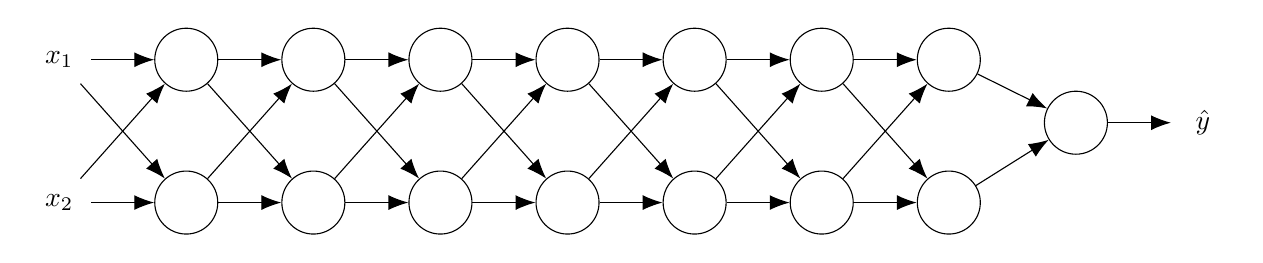
\begin{tikzpicture}[
    >={Latex[scale=1.5]},
    % Define the style for the nodes
    xory/.style={circle, minimum size=0.8cm, inner sep=0pt},
    neuron/.style={circle, draw=black, minimum size=0.8cm, inner sep=0pt},
    layer/.style={anchor=center, nodes=neuron, node distance=0.8cm}
]

% Input layer
\node[xory] (x1-1) {$x_1$};
\node[xory, below=of x1-1] (x1-2) {$x_2$};

% Hidden layers
\foreach \i [remember=\i as \lasti (initially 1)] in {2,...,8} {
    \node[neuron, right=0.8cm of x\lasti-1] (x\i-1) {};
    \node[neuron, below=of x\i-1] (x\i-2) {};
    \foreach \j in {1,2} {
        \foreach \k in {1,2} {
            \draw[->] (x\lasti-\k) -- (x\i-\j);
        }
    }
}

% Output layer
\node[neuron, right=0.8cm of x8-1, yshift=-0.8cm] (output) {};
\foreach \j in {1,2} {
    \draw[->] (x8-\j) -- (output);
}

\node[xory, right=0.8cm of output] (y-hat) {$\hat{y}$};
\draw[->] (output) -- (y-hat);

\end{tikzpicture}


This network has weights 
\[ w^1, w^2, \ldots, w^L \]

For the example we use a linear activation function
\[ g(z)=z \]

and set
\[ b^{[l]}=0 \]

Then we will have
\[ 
    \hat{y} = w^{[L]}w^{[L-1]} \times \ldots \times w^{[3]} w^{[2]} w^{[1]} x = w^{[L]} ( \prod_{l=1}^{L-1}w^{[l]})?x
\]

Now if
\[ 
    w^{[l]} =
    \begin{pmatrix}
        1.5 & 0 \\
        0 & 1.5 
    \end{pmatrix}
\]

Then for $\hat{y}$, the factor
\[
    \prod_{l=1}^{L-1}w^{[l]} = 
    \begin{pmatrix}
        1.5^{L-1} & 0 \\
        0 & 1.5^{L-1} 
    \end{pmatrix}
\]
and for large L, $1.5^{L-1}$ will become very large, and $\hat{y}$ will become very large.

Similarly, if we have
\[ 
    w^{[l]} =
    \begin{pmatrix}
        0.5 & 0 \\
        0 & 0.5 
    \end{pmatrix}
\]

Then for $\hat{y}$, the factor
\[
    \prod_{l=1}^{L-1}w^{[l]} = 
    \begin{pmatrix}
        0.5^{L-1} & 0 \\
        0 & 0.5^{L-1} 
    \end{pmatrix}
\]
and for large L, $0.5^{L-1}$ will become very small, and $\hat{y}$ will become very small.

So we have ($I$ being the identity matrix) that if
\[ w^{[l]} > I, \text{then with a deep network the activations can explode} \]
\[ w^{[l]} < I, \text{then with a deep network the activations can vanish} \]

A similar argument can be used to show that the derivatives or gradients will also increase 
or decrease exponentially as a function of the number of layers.


\subsection*{Weight Initialization for Deep Networks}

\begin{tikzpicture}[
    >={Latex[scale=2]},
    % Define the style for the nodes
    xory/.style={circle, minimum size=0.8cm, inner sep=0pt},
    neuron/.style={circle, draw=black, minimum size=0.8cm, inner sep=0pt},
    layer/.style={anchor=center, nodes=neuron, node distance=0.8cm}
]

\node[xory] (x1) {$x_1$};
\node[xory, below=0.7cm of x1] (x2) {$x_2$};
\node[xory, below=0.7cm of x2] (x3) {$x_3$};
\node[xory, below=0.7cm of x3] (x4) {$x_4$};
\node[neuron, right=2cm of x2, yshift=-0.7cm] (n1) {};
\node[xory, below=0.5cm of n1] (formula) {$a=g(z)$};
\node[xory, right=1.5cm of n1] (y1) {$\hat{y}$};

\draw[->] (x1) -- (n1);
\draw[->] (x2) -- (n1);
\draw[->] (x3) -- (n1);
\draw[->] (x4) -- (n1);
\draw[->] (n1) -- (y1);
    
\end{tikzpicture}


\[ z = w_1 x_1 + w_2 x_2 + \ldots + w_n x_n \]

so when $n \uparrow$, we want $w_i \downarrow$, in order not to have z grow too large.

One way of doing this is to make

\[ Var(w)= \frac{1}{n} \]

Do this by setting

\[ 
    w^{[l]} = 
    [rand(0 \ldots 1)] \times \sqrt{\frac{1}{n^{[l-1]}}} 
\]

where $[rand(0 \ldots 1)]$ is a random number between 0 and 1. This is called Xavier-initialization, 
and works well for the $tanh(z)$ activation function.

If using the ReLU activation function, using

\[ 
    w^{[l]} = 
    [random\ weight\ matrix] \times \sqrt{\frac{2}{n^{[l-1]}}} 
\]

has been found to work slightly better.

Another version is

\[
    w^{[l]} =
    [random\ weight\ matrix] \times \sqrt{\frac{2}{n^{[l-1]}+ n^{[l]}}}
\]

This could be made part of the hyperparameters to tune, but it's not the most important one.


\newpage



\subsection*{Gradient Checking}

Take all parameters $W^{[1]} , b^{[1]}, \ldots, W^L, b^L$  and reshape into a big vector $\theta$.

You will now have a cost function $\mathcal{J}(\theta)$

In the same way, gather all gradients $dW^{[1]} , db^{[1]}, \ldots, dW^L, db^L$ and reshape into a big vector $d\theta$.

We can now set

\[ 
    d\theta_{approx}^{[i]} = 
    (
        \mathcal{J}(\theta_1, \ldots, \theta_i + \epsilon, \ldots) 
        - 
        \mathcal{J}(\theta_1, \ldots, \theta_i - \epsilon, \ldots)  
    ) 
    / 
    2\epsilon
\]

We then do

\begin{algorithm}
    \caption*{Gradient Checking}
    \begin{algorithmic}[1]
        \Function{Check}{$d\theta_{approx}, d\theta, \epsilon$}
            \State \Return $\frac{||d\theta_{approx} - d\theta||_2}{||d\theta_{approx}||_2 + ||d\theta||_2} < \epsilon$
        \EndFunction

        \Statex
        
        \For {$i = 1$ to $n$}
            \State $Ok \gets$ \Call{Check}{$d\theta_{approx}^{[i]}, d\theta^{[i]}, 10^{-7}$}
        \EndFor
    \end{algorithmic}
\end{algorithm}		


\subsection*{Grad Check Implementation Notes}
\begin{itemize}
	\item Don't use in training - only to debug
	\item If grad check fails, look at the different components of $\theta$ to try to identify the bug. E.g. is it $dW$ or $db$ that is the problem?
	\item Remember the regularization term.
	\item Doesn't work with dropout.
	\item Run after random initialization (small $W, dW$), then again later after training for a while (larger $W, dW$). Errors might not show when the gradient is small.
\end{itemize}



% -----------------------------------------------------
% CHAPTER 2
% -----------------------------------------------------

\chapter{Week 2 \\ Optimization Algorithms}




% -- Mini-Batch Gradient Descent ------------------------------------------------

\section{Mini-Batch Gradient Descent}

\subsection*{Batch vs. Mini-Batch}

Vectorization allows you to efficiently compute on m examples.
\[ \underset{(n_X, m)}{X} = [x_1, \ldots, x_m] \]
\[ \underset{(1, m)}{Y} = [y_1, \ldots, y_m] \]

What if $m=5,000,000$?

We create batches:
\[ X^{\{1\}}= [x_1,\ldots, x_{1000} ] \]
\[ X^{\{2\}}= [x_{1001},\ldots, x_{2000} ] \]
\[ \vdots \]
\[ X^{\{5000\}}= [x_{4,999,001},\ldots, x_{5,000,000}] \]

and
\[  Y^{\{1\}}= [y_1,\ldots, y_{1000}] \]
\[  Y^{\{2\}}= [y_{1001},\ldots, y_{2000}] \]
\[  \vdots \]
\[  Y^{\{5000\}}= [y_{4,999,001},\ldots, y_{5,000,000}] \]

Now \textit{mini-batch} $t$ will be
\[ (X^{t} , T^{t}) \]

\newpage

\subsection*{Mini-Batch Gradient Descent}

Running one epoch (single pass over the whole training set):

\begin{algorithm}
    \caption*{Mini-Batch Gradient Descent}
    \begin{algorithmic}[1]
    \For{$t = 1$ to $5000$}

        \BlockComment{Forward propagation on $X^{\{t\}}$}
        \State $Z^{[1]} = W^{[1]}X^{\{t\}} + b^{[1]}$
        \State $A^{[1]} = g^{[1]}(Z^{[1]})$
        \State $\ldots$
        \State $Z^{[L]} = W^{[L]}A^{[L-1]} + b^{[L]}$
        \State $A^{[L]} = g^{[L]}(Z^{[L]})$
        
        \BlockComment{Compute cost on $Y^{\{t\}}$}
        \State $\mathcal{J}^{\{t\}} = \frac{1}{m} \sum_{i=1}^{m} \mathcal{L}(\hat{y}^{(i)}, y^{(i)}) + \frac{\lambda}{2m} \sum_{l=1}^{L} ||W^{[l]}||_F^2$ 

        \BlockComment{Backward propagation on $\mathcal{J}^{\{t\}}$}
        \State $dW = \ldots$    
        \State $db = \ldots$
        
        \BlockComment{Update parameters}
        \State $W^{[l]} = W^{[l]} - \alpha dW^{[l]}$
        \State $b^{[l]} = b^{[l]} - \alpha db^{[l]}$
    \EndFor
    \end{algorithmic}
\end{algorithm}

\newpage

\subsection*{Understanding and Training with Mini-batch Gradient Descent}

When training on a whole data set, the cost should decrease with each iteration.

When training on mini-batches, in each iteration we calculate $\mathcal{J}^t$  using $X^t$  and $Y^t$, so on each iteration we calculate the cost on a different data set. Hence we can expect the cost to trend downwards, but not to decrease on every iteration.

\begin{figure}[htbp]
    \begin{minipage}[t]{\textwidth}
        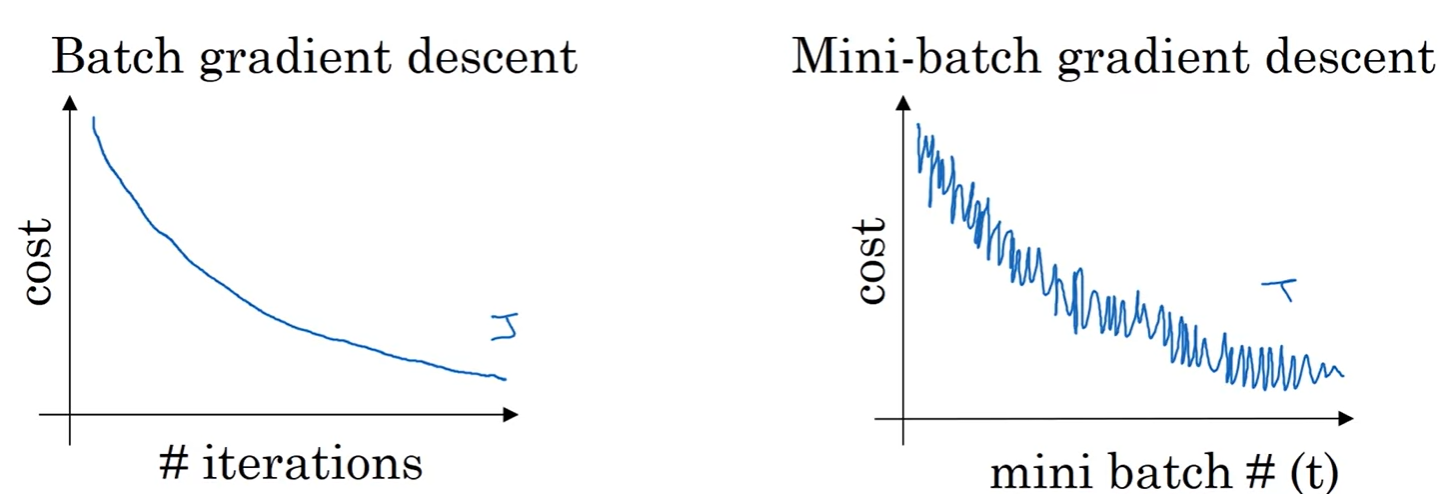
\includegraphics[width=\linewidth]{images/batch_vs_minibatch_gd.png}
    \end{minipage}
\end{figure}

\subsubsection*{Choosing the Mini-Batch Size}

If $m_{batch}=m$, then we have batch gradient descent and $(X^{\{t\}}, Y^{\{t\}} )=(X, Y)$. This is impractical for large data sets. \\
If $m_{batch}=1$, then we have stochastic gradient descent and $(X^{\{t\}}, Y^{\{t\}} )=(x^{(t)},y^{(t)} )$. This takes a long time to converge.

\begin{figure}[htbp]
    \begin{minipage}[t]{\textwidth}
        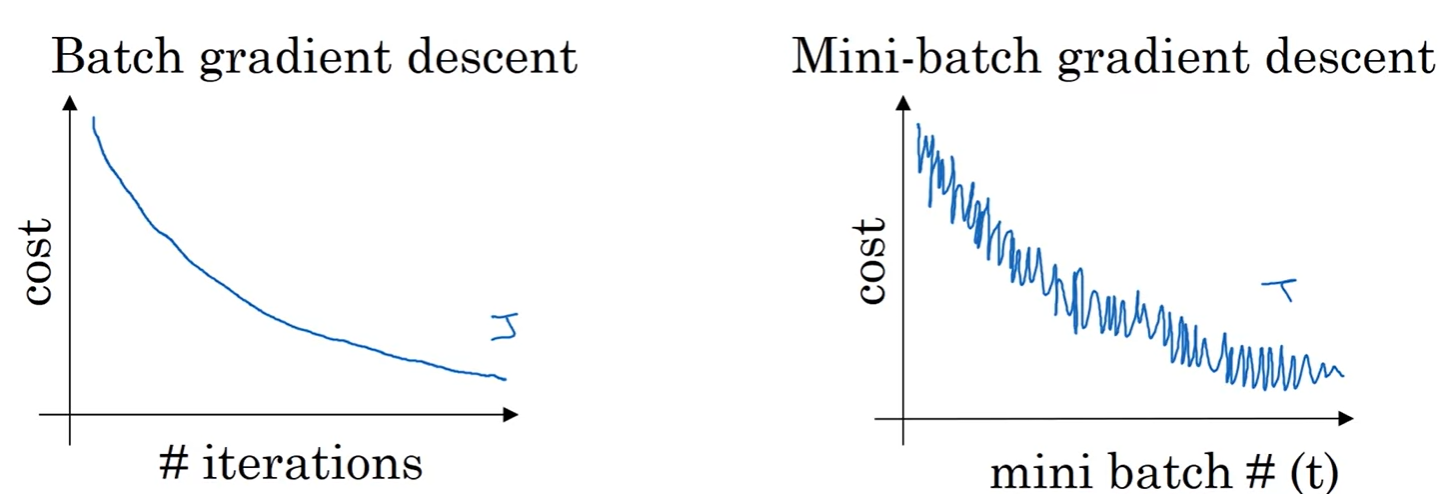
\includegraphics[width=\linewidth]{images/batch_vs_minibatch_gd.png}
        \end{minipage}
\end{figure}

Batch gradient descent
\begin{itemize}
    \item will converge faster
	\item take a (too) long time per iteration
\end{itemize}
	
Stochastic gradient descent:
\begin{itemize}
    \item will "wander around" more, taking steps in different directions depending on the single example that was used in that step
	\item lose the speedup gained by vectorization
\end{itemize}
	

In practice, for mini-batch gradient descent: $1<m_{batch}<m$
\begin{itemize}
    \item get perf gain from vectorization
	\item make progress without needing to wait for the entire training set to be processed
\end{itemize}

\subsection*{How to choose the batch size?}

If the training set is small $(m<2000)$: Use batch gradient descent.
Otherwise, typical mini-batch sizes are 64, 128, 256, 512 and sometimes (1024).

Make sure that the minibatch fits in memory (CPU or GPU) 





% -- Exponentially Weighted Averages -------------------------------------------

\section{Exponentially Weighted Averages}

Given a series of temperatures

\begin{tabular}{ |l|l| }
    \hline
    $\theta_1$ & 4 \\
    \hline
    $\theta_2$ & 9 \\
    \hline
    $\theta_3$ & 6 \\
    \hline
    $\vdots$ & $\vdots$ \\
    \hline
    $\theta_{180}$ & 15 \\
    \hline
    $\theta_{181}$ & 12 \\
    \hline
    $\vdots$ & $\vdots$ \\
    \hline
\end{tabular}

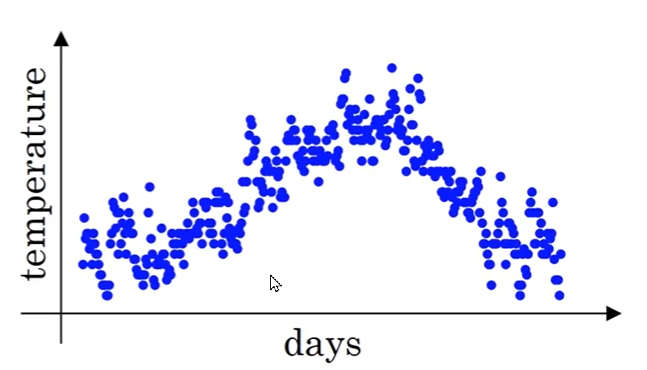
\includegraphics[width=0.7\linewidth]{images/temperatures.png}

Calculate a moving average

\begin{align*}
    V_0 &= 0 \\
    V_1 &= 0.9 V_0 + 0.1 \theta_1 \\
    V_2 &= 0.9 V_1 + 0.1 \theta_2 \\
        & \vdots \\
    V_t &= 0.9 V_{t-1} + 0.1 \theta_t 
\end{align*}

Plotting V in red gives:

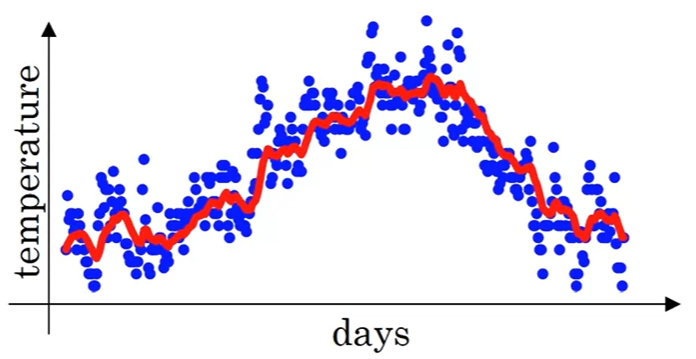
\includegraphics[width=0.7\linewidth]{images/temperatures_one_moving_avg.png}

More generally, we write

\[
    V_t = \beta V_{t-1} + (1 - \beta) \theta_t
\]

We can think of $V_t$  as approximately averaging over  $1/(1-\beta)$  days temperature, 
so for $\beta = 0.9$, we get an average over $1/(1 - 0.9) \approxeq 10$ days.

If we instead use $\beta = 0.98$, we get an average over $1/(1 - 0.98) \approxeq 50$ days, plotted in green below:

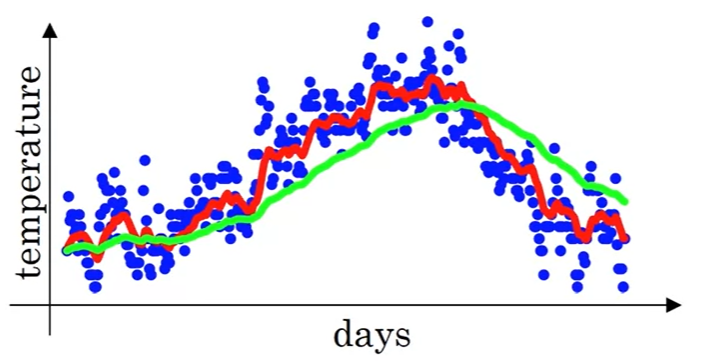
\includegraphics[width=0.7\linewidth]{images/temperatures_two_moving_avgs.png}

The curve is smoother since we are averaging over more values, but have also shifted to the right,
since it ``reacts'' more slowly to changes in temperature (most emphasis is placed on the $V_{t - 1}$ term.)

If we instead use $\beta = 0.5$, we get an average over $ 1 / (1 - 0.5) \approxeq 2$ days, plotted in yellow below:

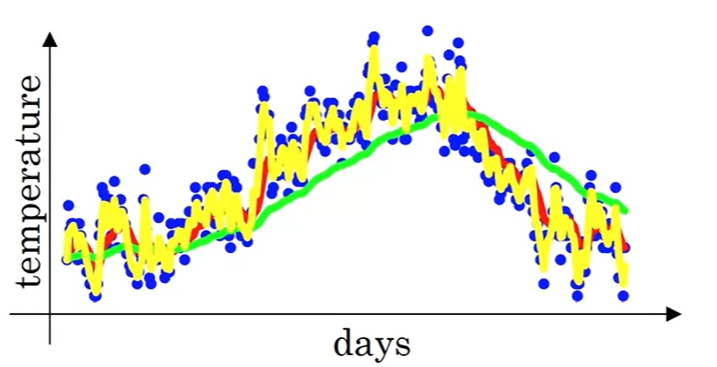
\includegraphics[width=0.7\linewidth]{images/temperatures_three_moving_avgs.png}


\subsection*{Understanding Exponentially Weighted Averages}

\begin{align*}
    V_100 &= 0.9V_{99} + 0.1 \theta_{100} \\
    V_99  &= 0.9V_{98} + 0.1 \theta_{99} \\
    V_98  &= 0.9V_{97} + 0.1 \theta_{98} \\
          & \vdots 
\end{align*}

\begin{align*}
    V_{100} & = 0.1 \theta_{100} + 
                0.9 (0.1 \theta_{99} + 0.9(0.1 \theta_{98} + 0.9(\ldots))) \\
            & = 0.1 (\theta_{100} + 0.9 \theta_{99} +0.9^2 \theta_{98} +0.9^3 \theta_{97} + 0.9^4 \theta_{96} + \ldots) \\
\end{align*}

So the weights of $\theta_n$ are decreasing exponentially.

We have that 
\[
    (1-\epsilon)^{1 / \epsilon} \approxeq 1/e \approxeq 0.35
\]

If we use $1 - \beta$ for $\epsilon$ in the above, we see that when going back $1 / (1 - \beta)$  time points, 
the weight has decreased to $1/e \approxeq 0.35$, which is why we say that we are averaging over that many time points.

\subsection*{Implementing Exponentially Weighted Averages}

Just initialize $V_{\theta}$ to $0$ and keep using it

\begin{align*}
    V_{\theta} &:= 0 \\
    V_{\theta} &:= \beta V_{\theta} + (1 - \beta) \theta_1 \\
    V_{\theta} &:= \beta V_{\theta} + (1 - \beta) \theta_2 \\
    V_{\theta} &:= \beta V_{\theta} + (1 - \beta) \theta_3 \\
    & \ldots 
\end{align*}

\subsection*{Bias Correction in Exponentially Weighted Averages}

For small values of $t$, $V_t$ is biased towards $0$. To overcome this, we introduce a bias factor $1 / (1 - \beta^t )$:
\[
    V_t^{'} = \frac{1}{1 - \beta^t} \cdot V_t = \frac{1}{1 - \beta^t} \cdot (\beta V_{t - 1} + (1 - \beta) \cdot \theta_t)
\]

With $\beta = 0.9, V_0 = 0$:

\begin{align*}
    V_1^{'} &= \frac{1}{1 - 0.9}  \cdot (0.9V_0 + 0.1 \theta_1 ) = \theta_1 \\
    V_2^{'} &= \frac{1}{1 - 0.9^2} \cdot (0.9V_1 + 0.1 \theta_2 )  \\
            &= \frac{1}{1 - 0.9^2} \cdot (0.9 \cdot (0.9V_0 + 0.1 \theta_1 ) + 0.1 \theta_2 )  \\
            &= \frac{1}{0.19} \cdot (0.09 \theta_1 + 0.1 \theta_2 ) = \underline{0.473 \cdot \theta_1 + 0.526 \cdot \theta_2} \\
\end{align*}





% -- Gradient Descent with Momentum --------------------------------------------

\section{Gradient Descent with Momentum}

Use an exponentially weighted average of the gradients to update the weights.

Ordinary gradient descent might "jump around" on its path towards the minimum (blue), 
or even diverge (purple), forcing you to use a small learning rate in order to have it converge.

\includegraphics*[width=0.7\linewidth]{images/gd_without_momentum.png}

We now intruduce momentum, which will dampen the oscillations and allow us to use a larger learning rate.

On iteration t, we compute the gradient $dW, db$ on the current mini-batch, then calculate
\[ V_{dW} =\beta V_{dW} + (1 - \beta) dW \]
\[ V_{db} =\beta V_{db} + (1 - \beta) db \]

We then update the weights:
\[ W \gets W - \alpha V_{dW} \]
\[ b \gets b - \alpha V_{db} \]

This will result in averaging out the gradients, making the algorithm head more directly towards the minimum (in red):

\includegraphics*[width=0.7\linewidth]{images/gd_with_momentum.png}

If we look at gradient descent's path towards the minimum as a ball rolling down the walls of a bowl 
towards the bottom, then in the equations above, e.g.
\[ V_{dW} = \beta V_{dW} + (1 - \beta) dW \]

we can view

\begin{itemize}
	\item the derivative term $dW$ as an acceleration term
	\item the momentum term $V_{dW}$  as the velocity
	\item $\beta$ as a friction factor, preventing unlimited speedup
\end{itemize}
    
In practice, $\beta = 0.9$ seems to work well, and bias correction is rarely used.

A version of momentum sometimes used is
\[ V_{dW} = \beta V_{dW} + dW \]
\[ V_{db} = \beta V_{db} + db \]

where the factor $(1 - \beta)$  has been omitted. The effect is that $V_{dW}$  and $V_{db}$  are scaled 
by a factor $( - \beta)$, and this need to be compensated for in the weight update by setting 
the learning rate $\alpha$ accordingly. A downside of this is that it entangles the hyperparameters $\alpha$ and $\beta$.




% -- RMSprop ------------------------------------------------------------------

\section{RMSprop}

An alternative to Gradient Descent with Momentum is RMSprop (Root Mean Square prop). The idea is to use an exponentially weighted 
average of the squared gradients to update the weights.

On iteration t, we compute the gradient $dW, db$ on the current mini-batch, then calculate

\[ S_{dW} =\beta S_{dW} + (1 - \beta) dW^2 \]
\[ S_{db} =\beta S_{db} + (1 - \beta) db^2 \]

We then update the weights:

\[ W \gets W - \alpha \frac{dW}{\sqrt{S_{dW}}} \]
\[ b \gets b - \alpha \frac{db}{\sqrt{S_{db}}} \]

The S expressions can be seen as exponentially weighted average of the squares of the derivatives.

What we want here is that in the example above, is that $S_{dW}$  will be small, so that in the update of 
$W$ we will divide $dW$ with a small value and take a big step, and that $S_{db}$  will be large,
so that in the update of $b$ we will divide $db$ with a large value and take a small step. 

This will result in a path towards the minimum that is more direct than with ordinary gradient descent.

In practice, to avoid division by $0$, a small term $\epsilon \approx 10^{-8}$  is introduced in the updates:

\[ W \gets W - \alpha \frac{dW}{\sqrt{S_{dW}} + \epsilon} \]
\[ b \gets b - \alpha \frac{db}{\sqrt{S_{db}} + \epsilon} \]




% -- Adam Optimization Algorithm -----------------------------------------------

\section{Adam Optimization Algorithm}

Like momentum and RMSprop, works well across many deep learning architectures.

Adam (Adaptive moment estimation) puts together momentum and RMSrop and combine them in one algorithm:

Set 
\begin{align*}
    V_{dW} & \gets 0 \\
    S_{dW} & \gets 0 \\
    V_{db} & \gets 0 \\
    S_{db} & \gets 0
\end{align*}

On iteration t, we compute the gradient $dW, db$ on the current mini-batch, then calculate
\begin{align*}
    V_{dW} &= \beta_1 V_{dW} + (1 - \beta_1) dW \\
    V_{db} &= \beta_1 V_{db} + (1 - \beta_1) db \\
    S_{dW} &= \beta_2 S_{dW} + (1 - \beta_2) dW^2 \\
    S_{db} &= \beta_2 S_{db} + (1 - \beta_2) db^2 
\end{align*}

Bias correction is typically used in Adam optimization, so we also calculate
\begin{align*}
    V_{dW}^{corrected} &= \frac{V_{dW}}{1 - \beta_1^t} \\
    V_{db}^{corrected} &= \frac{V_{db}}{1 - \beta_1^t} \\
    S_{dW}^{corrected} &= \frac{S_{dW}}{1 - \beta_2^t} \\
    S_{db}^{corrected} &= \frac{S_{db}}{1 - \beta_2^t} 
\end{align*}

We then update the weights:
\begin{align*}
    W & \gets W - \alpha \frac{V_{dW}^{corrected}}{\sqrt{S_{dW}^{corrected}} + \epsilon} \\
    b & \gets b - \alpha \frac{V_{db}^{corrected}}{\sqrt{S_{db}^{corrected}} + \epsilon} 
\end{align*}

Recommended values for hyperparameters:
\begin{tabular}{|l|l|}
    \hline
    $\alpha$ & needs to be tuned \\
    \hline
    $\beta_1$ & 0.9 \\
    \hline
    $\beta_2$ & 0.999 \\
    \hline
    $\epsilon$ & $10^{-8}$ \\
    \hline
\end{tabular}




% -- Learning Rate Decay -------------------------------------------------------

\section{Learning Rate Decay}

With a constant learning rate, the algorithm might get close to the minimum, but keep wandering around it and never really converge:

\includegraphics*[width=0.7\linewidth]{images/gd_no_lr_decay.png}

If instead you slowly reduce the learning rate during training, you end up taking smaller and smaller steps, bringing you closer to the minimum (in green):

\includegraphics*[width=0.7\linewidth]{images/gd_with_lr_decay.png}

A popular way of implemtning learning rate decay is to use the following formula:

\begin{align*}
    \alpha &= \frac{1}{1+decayRate \cdot epochNumber} \alpha_0 & & \text{(exponential decay)} \\
\end{align*}

where $\alpha_0$ is the initial learning rate, $decayRate$ is a hyperparameter and $epochNumber$ is the number of epochs.

With $\alpha_0 = 0$, $decayRate = 1$:

\begin{tabular}{|c|c|}
    \hline
    Epoch & $\alpha$ \\
    \hline
    1 & 0.1 \\
    \hline
    2 & 0.067 \\
    \hline
    3 & 0.05 \\
    \hline
    4 & 0.04 \\
    \hline
    \vdots & \vdots \\
    \hline
\end{tabular}

Other methods include :

\begin{align*}
    \alpha & = (0.95)^{epochNumber}\alpha_0           & &\text{(exponential decay)} \\
    \alpha &= \frac{k}{\sqrt{epochNumber}} \alpha_0   & &\text{(inverse decay)} \\
    \alpha &= \frac{k}{\sqrt{t}}                       & &\text{(discrete decay on every minibatch)} \\
\end{align*}

where $t$ is the minibatch number, and $k$ is a hyperparameter that need to be tuned.

Finally, manual tuning of the learning rate is sometimes used.





% -- The Problem of Local Optima ------------------------------------------------

\section{The Problem of Local Optima}

A worry when training a neural network could be that the algorithm gets stuck in a local minimum instead of the global minimum:

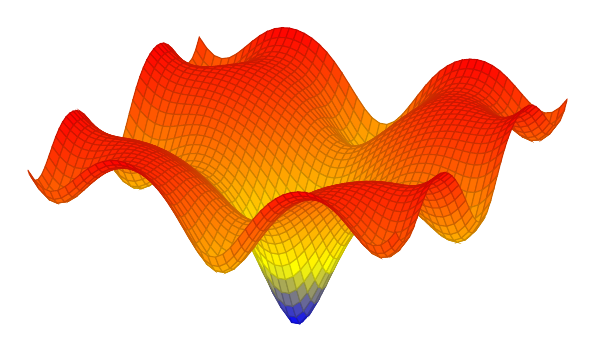
\begin{tikzpicture}
    \begin{axis}[
        xlabel={$x$},
        ylabel={$y$},
        zlabel={$f(x,y)$},
        ticks=none,
        samples=50,
        hide axis           
        ]
        \addplot3[surf, domain=-1.1:1.1, domain y=-1.1:1.1] {
            % Ackley's function
            -20*exp(-0.2*sqrt(0.5*(x^2+y^2))) - exp(0.5*(cos(deg(2*pi*x))+cos(deg(2*pi*y)))) + exp(1) + 20
            };
    \end{axis}
\end{tikzpicture}


As it turns out, neural networks operate in very high dimensional spaces, and there local minima are quite rare, 
it is much more likely that a point where the derivative is $0$ is a saddle point.

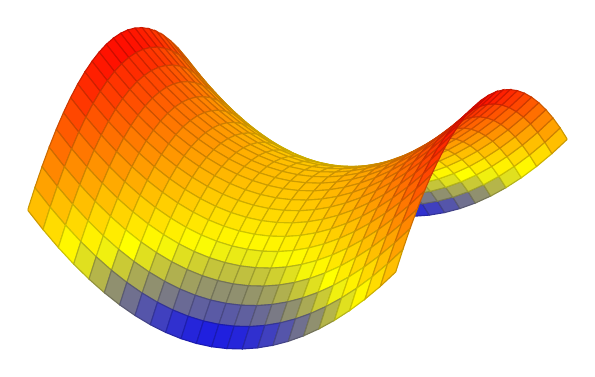
\begin{tikzpicture}
    \begin{axis}[
        xlabel={$x$},
        ylabel={$y$},
        zlabel={$f(x,y)$},
        ticks=none,
        hide axis
    ]
    \addplot3[surf, domain=-2:2, domain y=-2:2] {x^2-y^2};
    \end{axis}
\end{tikzpicture}

The reason for this is that for a point with derivative 0 to be a minimum, the function needs to be concave in all dimensions in that point, which is very unlikely in high dimensional spaces.

A more likely problem to encounter is plateaus, where the algorithm ends up traveling slowly across an almost flat "surface":

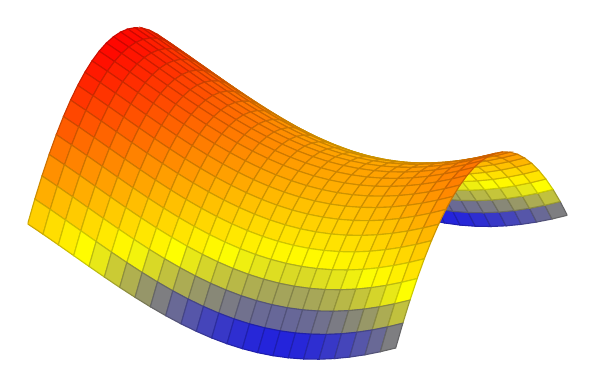
\begin{tikzpicture}
    \begin{axis}[
        xlabel={$x$},
        ylabel={$y$},
        zlabel={$f(x,y)$},
        ticks=none,
        hide axis
    ]
    \addplot3[surf, domain=-4:2, domain y=-2:2] {(x/2)^2 - (x/4)^4 - (1*y)^2};
    \end{axis}
\end{tikzpicture}


\chapter{Week 3 \\ Hyperparameter Tuning}


% - Hyperparameter Tuning -------------------------------------------------------
\section{Hyperparameter Tuning}

Parameters to tune:
\begin{tabular}{|l|l|}
    \hline
    Parameter & Priority \\
    \hline
    $\alpha$ & 1 \\
    \hline
    $\beta$ & 2 \\
    \hline
    $\beta_1, \beta_2, \epsilon$ & 4 \\
    \hline
    numLayers & 3 \\
    \hline
    numHiddenUnits & 2 \\
    \hline
    learningRateDecay & 3 \\
    \hline
    miniBatchSize & 2 \\
    \hline
\end{tabular}

\subsection*{Tuning Parameters}

\subsubsection*{Random Sampling}

Selecting values to try from a grid used to be common practice:
\begin{tikzpicture}
    % Draw square
    \draw (0,0) rectangle (7,7);
    
    % Add labels
    \node[rotate=90, anchor=center] at (-0.5,3.5) {Hyperparameter 1};
    \node[anchor=center] at (3.5,7.5) {Hyperparameter 2};
    
    % Draw the 5x5 grid inside the square
    \foreach \x in {1.4, 2.8, 4.2, 5.6} {
        \foreach \y in {1.4, 2.8, 4.2, 5.6} {
            \fill (\x,\y) circle (2pt);
        }
    }
\end{tikzpicture}

A better approach is to sample randomly:


\begin{tikzpicture}
    % Draw square
    \draw (0,0) rectangle (7,7);
    
    % Add labels
    \node[rotate=90, anchor=center] at (-0.5,3.5) {Hyperparameter 1};
    \node[anchor=center] at (3.5,7.5) {Hyperparameter 2};
    
    % Define the coordinates in an array
    \def\pointslist{
        (1,2), (5,5.5), (2.5,6.2), (6,1.5), (3.7,2.3), 
        (1.5,5), (2,1), (6.5,6), (5.5,1.5), (3,5.5),
        (4.5,3), (1.2,3.5), (6.2,4), (5.8,2.7), (2.2,4.6), 
        (4,6), (3.5,1.2), (6.5,3), (5,3.5), (1.8,6),
        (4,2.5), (2.5,2), (3.5,4.5), (4.8,5), (2.8,1.5)
    }
    
    % Loop through each coordinate and plot the point
    \foreach \point in \pointslist {
        \fill \point circle (2pt);
    }
\end{tikzpicture}

If only one of the parameters turns out to be unimportant, then at least with the random sampling we end up 
trying many more values for the important parameter.

\subsubsection*{Coarse to fine}

If after a coarse search in the space of all hyperparameters you find that the best combinations of values
lie in a smaller part of that space, zoom in to that subspace and and do a more fine grained search.


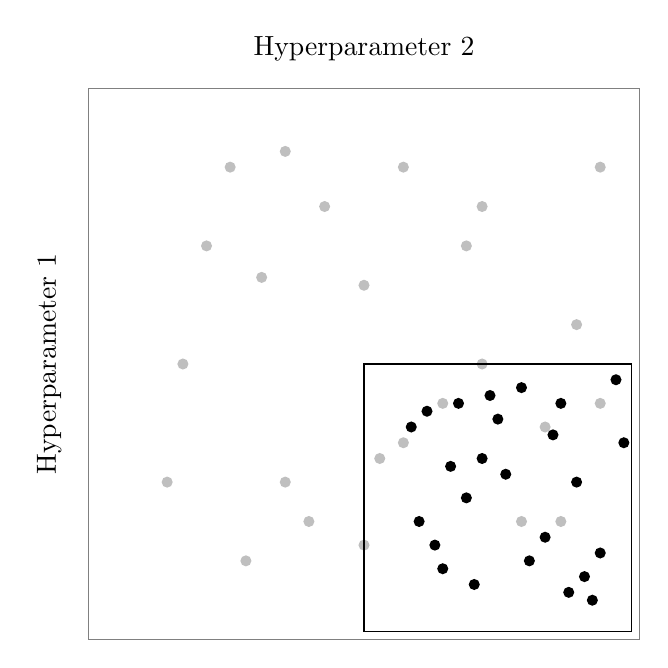
\begin{tikzpicture}
    % Draw square
    \draw[draw=gray] (0,0) rectangle (7,7);
    
    % Add labels
    \node[rotate=90, anchor=center] at (-0.5,3.5) {Hyperparameter 1};
    \node[anchor=center] at (3.5,7.5) {Hyperparameter 2};
    
    % Define the coordinates in an array
    \def\pointslist{
        (1,2), (5,5.5), (2.5,6.2), (6,1.5), (3.7,2.3), 
        (1.5,5), (2,1), (6.5,6), (5.5,1.5), (3,5.5),
        (4.5,3), (1.2,3.5), (6.2,4), (5.8,2.7), (2.2,4.6), 
        (4,6), (3.5,1.2), (6.5,3), (5,3.5), (1.8,6),
        (4,2.5), (2.5,2), (3.5,4.5), (4.8,5), (2.8,1.5)
    }
    
    % Loop through each coordinate and plot the point
    \foreach \point in \pointslist {
        \fill[fill=lightgray] \point circle (2pt);
    }

    \def\pointslistx{
    (4.2,1.5), (6.3,0.8), (5,2.3), (6.5,1.1), (4.7,3),
    (6.8,2.5), (4.9,0.7), (5.5,3.2), (4.3,2.9), (5.6,1),
    (5.3,2.1), (6.1,0.6), (6.7,3.3), (4.5,0.9), (6.2,2),
    (5.8,1.3), (6,3), (4.6,2.2), (4.1,2.7), (4.8,1.8),
    (5.2,2.8), (6.4,0.5), (5.1,3.1), (5.9,2.6), (4.4,1.2)
    }
 
    % Loop through each coordinate and plot the point
    \foreach \point in \pointslistx {
        \fill[fill=black] \point circle (2pt);
    }

    \draw[draw=black] (3.5,3.5) rectangle (6.9, 0.1);

\end{tikzpicture}

\section{Using an Appropriate Scale to pick Hyperparameters}

There are several ways to pick hyperparameters at random, depending on their scale.

\subsection*{Sampling uniformly at random }

Examples:

Number of hiddenunits in layer $l$: $n^{[l]} \in [50,100]$

Number of layers in a network, $L: L \in [2,4]$

\subsection*{Sampling from a logarithmic distribution}

Example:

Sample learning rate between $0.0001$ and $1$

\[ \{r | r \in \mathbb{R}, -4 \leq r \leq 0\} \]
\[ \alpha = 10^r \]

Generally, sampling a value $v$ between $10^a$  and $10^b$:

\[ \{ r | r \in \mathbb{R}, a \le r \le b\} \]
\[ v = 10^r \]

\subsection*{Sampling hyperparameters for exponentially weighted averages}

Sample $\beta$ between $0.9$ and $0.999$

Sample $(1 - \beta)$  from $0.1$ to $0.001$ (see log sampling above)


\section{Hyperparameters Tuning in Practice}

Intuitions can transfer between domains.
Intutions can go stale. Re-evaluate hyperparameters occasionally.

\subsection*{Babysitting one model}

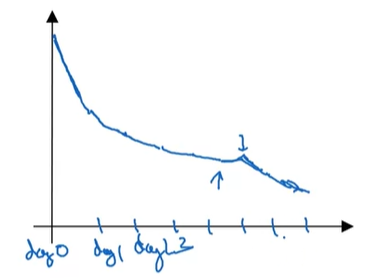
\includegraphics[width=0.3\linewidth]{images/single_model.png}

When training over a long time, adjust parameters as training progresses.

\subsection*{Training many models in parallel}

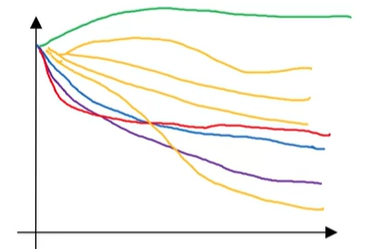
\includegraphics[width=0.3\linewidth]{images/parallel_models.png}

Allows you to test many parameter values at the same time, pick the best in the end.




% - Batch Normalization ---------------------------------------------------------

\section{Batch Normalization - Normalizing Activations in a Network}

\subsection*{Logistic regression}

For a single neuron we have seen how we can normalize the inputs

\begin{tikzpicture}[
    >={Latex[scale=2]},
    % Define the style for the nodes
    xory/.style={circle, minimum size=0.8cm, inner sep=0pt},
    neuron/.style={circle, draw=black, minimum size=0.8cm, inner sep=0pt},
    layer/.style={anchor=center, nodes=neuron, node distance=0.8cm}
]

    \node[xory] (x1) {$x_1$};
    \node[xory, below=0.7cm of x1] (x2) {$x_2$};
    \node[xory, below=0.7cm of x2] (x3) {$x_3$};
    \node[neuron, right=2cm of x2] (n1) {};
    \node[xory, right=0.5cm of x1] (formula) {$w,b$};
    \node[xory, right=1.5cm of n1] (y1) {$\hat{y}$};

    \draw[->] (x1) -- (n1);
    \draw[->] (x2) -- (n1);
    \draw[->] (x3) -- (n1);
    \draw[->] (n1) -- (y1);

\end{tikzpicture}

We calculate mean and variance:

\[ \mu = \frac{1}{m} \sum_{i=1}^m x^{(i)} \]
\[ \sigma^2 = \frac{1}{m} \sum_{i=1}^m (x^{(i)} - \mu)^2 \]

Then normalize $X$:

\[ \hat{X} = \frac{X - \mu}{\sqrt{\sigma^2 + \epsilon}} \]

\subsection*{Deeper Networks}

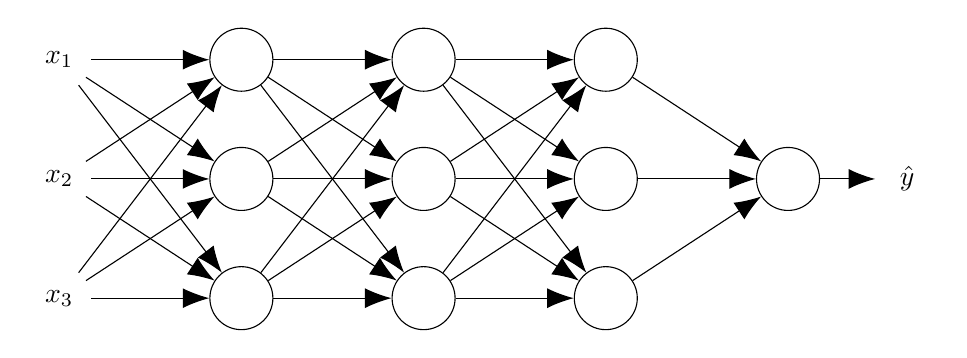
\begin{tikzpicture}[
    >={Latex[scale=2]},
    % Define the style for the nodes
    xory/.style={circle, minimum size=0.8cm, inner sep=0pt},
    neuron/.style={circle, draw=black, minimum size=0.8cm, inner sep=0pt},
    layer/.style={anchor=center, nodes=neuron, node distance=0.8cm}
]

    % input layer
    \node[xory] (x1-1) {$x_1$};
    \node[xory, below=0.7cm of x1-1] (x1-2) {$x_2$};
    \node[xory, below=0.7cm of x1-2] (x1-3) {$x_3$};

    % hidden layers
    \foreach \i [remember=\i as \lasti (initially 1)] in {2, 3, 4} {
        \node[neuron, right=1.5cm of x\lasti-1] (x\i-1) {};
         \node[neuron, right=1.5cm of x\lasti-2] (x\i-2) {};
         \node[neuron, right=1.5cm of x\lasti-3] (x\i-3) {};

         \foreach \j in {1,...,3} {
             \foreach \k in {1,...,3} {
                 \draw[->] (x\lasti-\k) -- (x\i-\j);
             }
         }
    }

    %output
    \node[neuron, right=1.5cm of x4-2] (y1) {};
    \draw[->] (x4-1) -- (y1);
    \draw[->] (x4-2) -- (y1);
    \draw[->] (x4-3) -- (y1);
    \node[xory, right=0.7cm of y1] (yhat) {$\hat{y}$};
    \draw[->] (y1) -- (yhat);

\end{tikzpicture}

For any hidden layer, can we normalize $a^{[l-1]}$  so as to train $w^{[l]}, b^{[l]}$ faster?

Given some intermediate values for a layer in a neural network $\{z^{(1)}, \ldots, z^{(m)}\}$, we can normalize them:
\begin{align*}
    \mu            &= \frac{1}{m} \sum_i z^{(i)} \\
    \sigma^2       &= \frac{1}{m} \sum_i(z^{(i)} - \mu)^2 \\
    z_{norm}^{(i)} &= \frac{z^{(i)} - \mu}{\sigma} \approx \frac{z^{(i)} - \mu}{\sqrt{\sigma^2+\epsilon}} 
\end{align*}

Now we don't always want the input to the activation functions to have mean $0$ and variance $1$, so we take
\[ \tilde{z}^{(i)}=\gamma z_{norm}^{(i)} + \beta \]

where $\beta, \gamma$ are learnable parameters of the model.

Now if
\[
\begin{cases}
    \gamma &= \sqrt{\sigma^2 + \epsilon} \\
    \beta  &= \mu
\end{cases}
\]

then
\[ \tilde{z}^{(i)} = z^{(i)} \]

so any mean and variance can be learned. Batch Norm also makes the constant $b$ in the expression 
$a=Wx+b$ redundant, since it will be removed in the normalization step. The $\beta$ term will play the same role as $b$ here.

When working with mini-batches, normalization is done over each mini-batch using only the data from that mini-batch.

\subsection*{Why does Batch Norm work?}

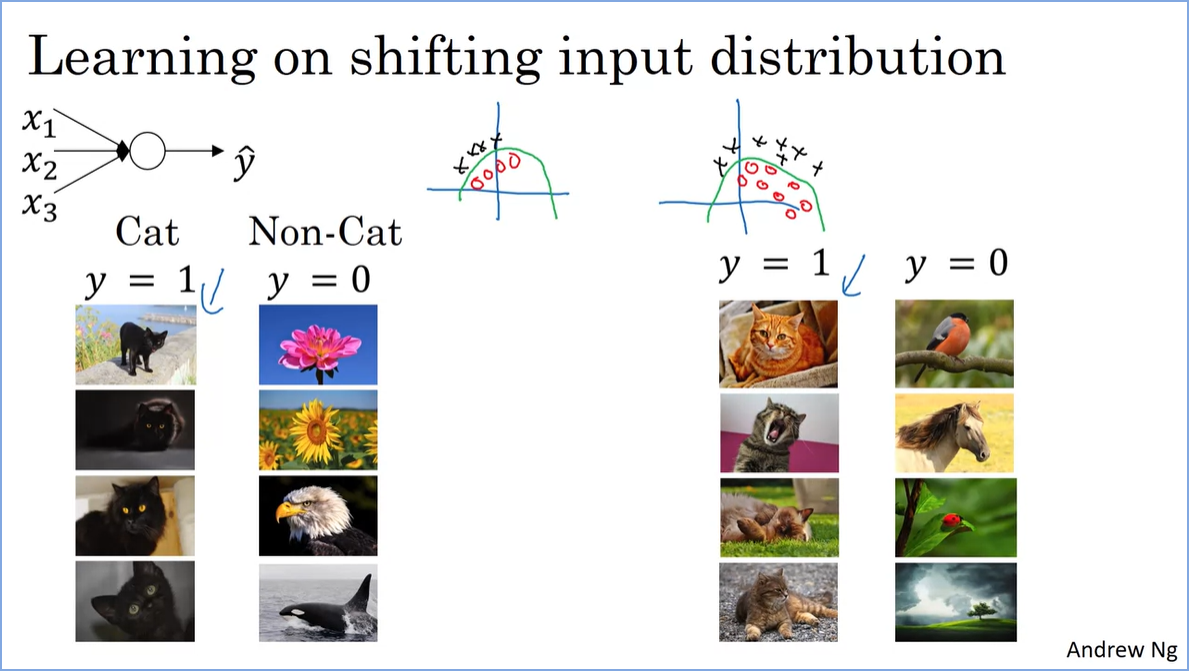
\includegraphics[width=\linewidth]{images/learning_on_shifting_distribution.png}

A function trained on the data set on the left will not be good at predicting labels in the data set on the right. 
They come from a shifted distribution, known as a covariate shift.

Covariate shift $\implies$ a need to retrain the network.

A layer deeper than the first of a DNN suffers from covariate shift due to the shifting inputs from the previous layers:

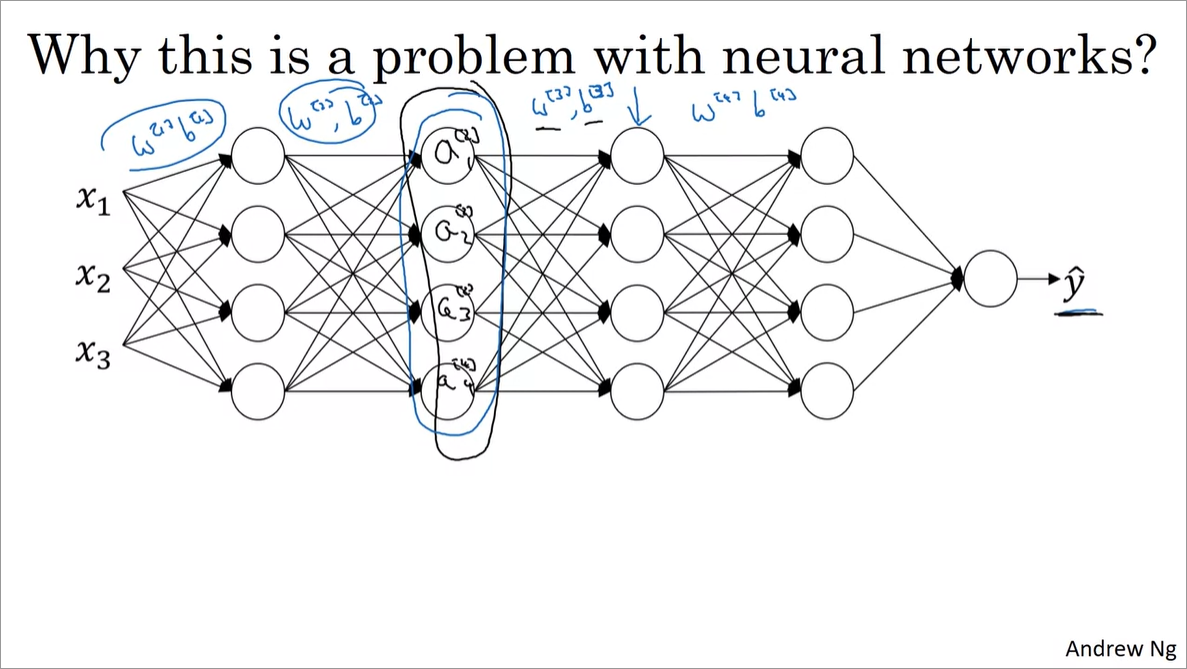
\includegraphics[width=\linewidth]{images/nn_covariate_shift.png}

Batch norm will address this by limiting the changes in the input to a layer since variance and mean will now remain the same.

\subsection*{Batch Norm As Regularization}

\begin{itemize}
    \item Each mini-batch is scaled by the mean/variance computed on just that mini-batch.
    \item This adds some noise to the values $z^{[l]}$ within that mini-batch. So similar to dropout, it adds some noise to each hidden layer's activations.
    \item This has a slight regularization effect.
\end{itemize}

\subsection*{Batch Norm at Test Time}

At test time, $\mu$ and $\sigma$ are estimated using exponential weighted averages across mini-batches, 
so during training you keep a running average of these variables.




% - Softmax Regression ----------------------------------------------------------
\section{Softmax Regression}

Generalization of logistic regression.

The output of the final layer $L$ with $C$ outputs is computed as usual
\begin{align*}
    z^{[L]} & = W^{[L]} a^{[L-1]} + b^{[L]}   & \text{matrix of dim}(4,1)
\end{align*}

Activation function for layer $L$:
\[ t = e^{(z^{[L]})} \]
\[ a^{[L]} = \frac{e^{z^{[L]}}}{\sum_{j=1}^C t_j},\ \ a_i = \frac{t_i}{ \sum_{j=1}^C t_j} \]

So if e.g.
\[
    z^{[L]} = 
    \begin{bmatrix}
        5 \\
        2 \\
        -1 \\
        3
    \end{bmatrix}
    \implies
    t =
    \begin{bmatrix}
        e^5 \\
        e^2 \\
        e^{-1} \\
        e^3
    \end{bmatrix}
    =
    \begin{bmatrix}
        148.4 \\
        7.4 \\
        0.4 \\
        20.1
    \end{bmatrix}
\]
\[ \sum_{i=1}^4 t_i = 176.3 \]
 \[
    a^{[L]} = 
    \begin{bmatrix}
        e^5/176.3 \\
        e^2/176.3 \\
        e^{-1}/176.3 \\
        e^3/176.3
    \end{bmatrix}
    =
    \begin{bmatrix}
        0.842 \\
        0.042 \\
        0.002 \\
        0.114
    \end{bmatrix}
    , \text{  hardmax would be}
    \begin{bmatrix}
        1 \\
        0 \\
        0 \\
        0
    \end{bmatrix}
\]

Softmax generalizes logistic regression to $C$ classes. If $C=2$, softmax reduces to logistic regression.

\subsection*{Loss Function}

The loss function used for softmax is
\[ \mathcal{L}(\hat{y}, y)= -\sum_{j=1}^Cy_j \cdot log(\hat{y}_j) \]

Example:
\[
    y = 
    \begin{bmatrix}
        0 \\
        1 \\
        0 \\
        0
    \end{bmatrix}
    ,
    a^{[L]} =
    \hat{y} =
    \begin{bmatrix}
        0.3 \\
        0.2 \\
        0.1 \\
        0.4 
    \end{bmatrix}    
\]

In this case the loss function will be
\[ \mathcal{L}(\hat{y}, y) = - y_2 \cdot log(\hat{y}_2) \]

The way to minimize this is to make $\hat{y}^2$ big, which is what we want. In this case we get
\[ \mathcal{L}(\hat{y}, y) = - log(0.2) = 1.61 \]

The cost function then becomes
\[
    \mathcal{J}(W,b) = \frac{1}{m} \sum_{i=1}^m \mathcal{L}(\hat{y}^{(i)}, y^{[i)}) \]

For the whole training set with $m$ examples, $Y$ is a matrix with dimensions $(4, m)$.

\subsection*{Gradient Descent}


\[
    dz^{[L]} = \partial{\mathcal{J}}{z^{[L]}} = \hat{y} - y 
\]

\section*{Deep Learning Frameworks}

\begin{itemize}
    \item Caffe/Caffe2
    \item CNTK
    \item DL4J
    \item Keras
    \item Lasagne
    \item mxnet
    \item PaddlePaddle
    \item TensorFlow
    \item Theano
    \item Torch
\end{itemize}

\subsection*{Choosing deep learning frameworks}

\begin{itemize}
    \item Ease of programming (development + deployment)
    \item Running speed
    \item Truly open (open source with good governance)
    \item Community support
    \item Hardware support (GPUs, CPUs, TPUs)
    \item Production support (ability to easily train huge models over multiple machines)
    \item Learning curve (easy to learn)
    \item Debugging and visualization tools
    \item Popularity
\end{itemize}


\end{document}